
\documentclass[journal,12pt,twocolumn]{IEEEtran}
%
\usepackage{setspace}
\usepackage{gensymb}
%\doublespacing
\singlespacing

%\usepackage{graphicx}
%\usepackage{amssymb}
%\usepackage{relsize}
\usepackage[cmex10]{amsmath}
%\usepackage{amsthm}
%\interdisplaylinepenalty=2500
%\savesymbol{iint}
%\usepackage{txfonts}
%\restoresymbol{TXF}{iint}
%\usepackage{wasysym}
\usepackage{amsthm}
%\usepackage{iithtlc}
\usepackage{mathrsfs}
\usepackage{txfonts}
\usepackage{stfloats}
\usepackage{bm}
\usepackage{cite}
\usepackage{cases}
\usepackage{subfig}
%\usepackage{xtab}
\usepackage{longtable}
\usepackage{multirow}
%\usepackage{algorithm}
%\usepackage{algpseudocode}
\usepackage[utf8]{inputenc}
\usepackage{tikz}
\usetikzlibrary{positioning}
\usepackage{enumitem}
\usepackage{mathtools}
\usepackage{steinmetz}
\usepackage{tikz}
\usepackage{circuitikz}
\usepackage{verbatim}
\usepackage{tfrupee}
\usepackage[breaklinks=true]{hyperref}
%\usepackage{stmaryrd}
\usepackage{tkz-euclide} % loads  TikZ and tkz-base
%\usetkzobj{all}
\usetikzlibrary{calc,math}
\usepackage{listings}
    \usepackage{color}                                            %%
    \usepackage{array}                                            %%
    \usepackage{longtable}                                        %%
    \usepackage{calc}                                             %%
    \usepackage{multirow}                                         %%
    \usepackage{hhline}                                           %%
    \usepackage{ifthen}                                           %%
  %optionally (for landscape tables embedded in another document): %%
    \usepackage{lscape}     
\usepackage{multicol}
\usepackage{chngcntr}
%\usepackage{enumerate}

%\usepackage{wasysym}
%\newcounter{MYtempeqncnt}
\DeclareMathOperator*{\Res}{Res}
%\renewcommand{\baselinestretch}{2}
\renewcommand\thesection{\arabic{section}}
\renewcommand\thesubsection{\thesection.\arabic{subsection}}
\renewcommand\thesubsubsection{\thesubsection.\arabic{subsubsection}}

\renewcommand\thesectiondis{\arabic{section}}
\renewcommand\thesubsectiondis{\thesectiondis.\arabic{subsection}}
\renewcommand\thesubsubsectiondis{\thesubsectiondis.\arabic{subsubsection}}

% correct bad hyphenation here
\hyphenation{op-tical net-works semi-conduc-tor}
\def\inputGnumericTable{}                                 %%

\lstset{
%language=C,
frame=single, 
breaklines=true,
columns=fullflexible
}
%\lstset{
%language=tex,
%frame=single, 
%breaklines=true
%}

\begin{document}
%


\newtheorem{theorem}{Theorem}[section]
\newtheorem{problem}{Problem}
\newtheorem{proposition}{Proposition}[section]
\newtheorem{lemma}{Lemma}[section]
\newtheorem{corollary}[theorem]{Corollary}
\newtheorem{example}{Example}[section]
\newtheorem{definition}[problem]{Definition}
%\newtheorem{thm}{Theorem}[section] 
%\newtheorem{defn}[thm]{Definition}
%\newtheorem{algorithm}{Algorithm}[section]
%\newtheorem{cor}{Corollary}
\newcommand{\BEQA}{\begin{eqnarray}}
\newcommand{\EEQA}{\end{eqnarray}}
\newcommand{\define}{\stackrel{\triangle}{=}}
\bibliographystyle{IEEEtran}
%\bibliographystyle{ieeetr}
\providecommand{\mbf}{\mathbf}
\providecommand{\pr}[1]{\ensuremath{\Pr\left(#1\right)}}
\providecommand{\qfunc}[1]{\ensuremath{Q\left(#1\right)}}
\providecommand{\sbrak}[1]{\ensuremath{{}\left[#1\right]}}
\providecommand{\lsbrak}[1]{\ensuremath{{}\left[#1\right.}}
\providecommand{\rsbrak}[1]{\ensuremath{{}\left.#1\right]}}
\providecommand{\brak}[1]{\ensuremath{\left(#1\right)}}
\providecommand{\lbrak}[1]{\ensuremath{\left(#1\right.}}
\providecommand{\rbrak}[1]{\ensuremath{\left.#1\right)}}
\providecommand{\cbrak}[1]{\ensuremath{\left\{#1\right\}}}
\providecommand{\lcbrak}[1]{\ensuremath{\left\{#1\right.}}
\providecommand{\rcbrak}[1]{\ensuremath{\left.#1\right\}}}
\theoremstyle{remark}
\newtheorem{rem}{Remark}
\newcommand{\sgn}{\mathop{\mathrm{sgn}}}
\providecommand{\abs}[1]{\ensuremath{\left\vert#1\right\vert}}
\providecommand{\res}[1]{\Res\displaylimits_{#1}} 
\providecommand{\norm}[1]{\ensuremath{\left\lVert#1\right\rVert}}
%\providecommand{\norm}[1]{\lVert#1\rVert}
\providecommand{\mtx}[1]{\mathbf{#1}}
\providecommand{\mean}[1]{\ensuremath{E\left[ #1 \right]}}
\providecommand{\fourier}{\overset{\mathcal{F}}{ \rightleftharpoons}}
%\providecommand{\hilbert}{\overset{\mathcal{H}}{ \rightleftharpoons}}
\providecommand{\system}{\overset{\mathcal{H}}{ \longleftrightarrow}}
	%\newcommand{\solution}[2]{\textbf{Solution:}{#1}}
\newcommand{\solution}{\noindent \textbf{Solution: }}
\newcommand{\cosec}{\,\text{cosec}\,}
\providecommand{\dec}[2]{\ensuremath{\overset{#1}{\underset{#2}{\gtrless}}}}
\newcommand{\myvec}[1]{\ensuremath{\begin{pmatrix}#1\end{pmatrix}}}
\newcommand{\mydet}[1]{\ensuremath{\begin{vmatrix}#1\end{vmatrix}}}
%\numberwithin{equation}{section}
\numberwithin{equation}{subsection}
%\numberwithin{problem}{section}
%\numberwithin{definition}{section}
\makeatletter
\@addtoreset{figure}{problem}
\makeatother
\let\StandardTheFigure\thefigure
\let\vec\mathbf
%\renewcommand{\thefigure}{\theproblem.\arabic{figure}}
\renewcommand{\thefigure}{\theproblem}
%\setlist[enumerate,1]{before=\renewcommand\theequation{\theenumi.\arabic{equation}}
%\counterwithin{equation}{enumi}
%\renewcommand{\theequation}{\arabic{subsection}.\arabic{equation}}
\def\putbox#1#2#3{\makebox[0in][l]{\makebox[#1][l]{}\raisebox{\baselineskip}[0in][0in]{\raisebox{#2}[0in][0in]{#3}}}}
     \def\rightbox#1{\makebox[0in][r]{#1}}
     \def\centbox#1{\makebox[0in]{#1}}
     \def\topbox#1{\raisebox{-\baselineskip}[0in][0in]{#1}}
     \def\midbox#1{\raisebox{-0.5\baselineskip}[0in][0in]{#1}}
\vspace{3cm}
\title{Assignment 8}
\author{Vishal Ashok}
\maketitle
\newpage
%\tableofcontents
\bigskip
\renewcommand{\thefigure}{\theenumi}
\renewcommand{\thetable}{\theenumi}
\begin{abstract}
This document uses the concepts of singular value decomposition in solving a problem.
\end{abstract}
Download Python code from 
%
\begin{lstlisting}
https://github.com/vishalashok98/AI5006/tree/master/Assignment3\end{lstlisting}
%
Download latex-tikz codes from 
%
\begin{lstlisting}
https://github.com/vishalashok98/AI5006/tree/master/Assignment3\end{lstlisting}
%
\section{Problem}
Find the foot of the perpendicular from the point  $\myvec{-1 \\ 2 \\ 4}$ to the plane 
\begin{align}
    2x + 3y - 4z +5 = 0  \label{given_plane_eq}
\end{align}
\section{Explanation}
The general equation of a plane is given by
\begin{align}
    px+by+cz = d \label{gen_plane_eqn}
\end{align}
and can be expressed as
\begin{align}
    \vec{n}^T\vec{x} = d \label{plane_vec_eqn}
\end{align}
where
\begin{align}
    \vec{n} = \myvec{p \\ q \\ r}
\end{align}
The equation of a line passing through the point $a$ and having direction vector $\vec{b}$ is given by
\begin{align}
    \vec{x} = \vec{a} +\lambda \vec{b} \label{vec_line_eq}
\end{align}
\section{Solution}
Writing the equation of given plane in \eqref{plane_vec_eqn} form, we get
\begin{align}\label{eq0}
	\myvec{2 & 3 & -4}\myvec{x\\y\\z} = -5
\end{align}
where :
$\vec{n}=\myvec{2\\ 3 \\-4}$, $\vec{x} = \myvec{x\\y\\z}$  and $c=-5$\\
We need to represent equation of plane in parametric form,
\begin{equation}\label{eq1}
	\vec{x} = \vec{p} + \lambda_1\vec{q} + \lambda_2\vec{r}
\end{equation}
Here $\vec{p}$ is any point on plane and $\vec{q}, \vec{r}$ are two vectors parallel to plane and hence $\perp$ to $\vec{n}$. Find two vectors that are $\perp$ to $\vec{n}$
\begin{align}\label{eq2}
	\implies\myvec{2 & 3 & -4}\myvec{a\\b\\c} = 0
\end{align}
Put $a=1$ and $b=0$ in \eqref{eq2}, $\implies c=\frac{1}{2}$\\
Put $a=0$ and $b=1$ in \eqref{eq2}, $\implies c=\frac{3}{4}$\\
Hence $\vec{q} = \myvec{1\\0\\\frac{1}{2}}, \vec{r} = \myvec{0\\1\\\frac{3}{4}}$\\
Let us find point $\vec{p}$ on the plane. Put $x=1,y=1$ in \eqref{eq0}, we get $\vec{p} = \myvec{0\\1\\\frac{5}{2}}$\\
Since given plane is perpendicular to given line, if we take $\vec{P} = \myvec{-1 \\ 2 \\ 4}$ it will give us the shortest distance to the plane. \\
Let $\vec{Q}$ be the point on plane with shortest distance to $\vec{P}$. $\vec{Q}$ can be expressed in \eqref{eq1} form as
\begin{align}\label{eq3}
	\vec{Q} = \myvec{1\\1\\\frac{5}{2}} + \lambda_1\myvec{1\\0\\\frac{1}{2}} + \lambda_2\myvec{0\\1\\\frac{3}{4}}
\end{align}
Equate $\vec{P}$ and $\vec{Q}$, and compute $\lambda_1, \lambda_2$ using $\textit{pseudoinverse}$ from $\textit{SVD}$
\begin{align}
	\myvec{1\\1\\\frac{5}{2}} + \lambda_1\myvec{1\\0\\\frac{1}{2}} + \lambda_2\myvec{0\\1\\ \frac{3}{4}} &= \myvec{-1\\2\\4}\\
	\lambda_1\myvec{1\\0\\\frac{1}{2}} + \lambda_2\myvec{0\\1\\ \frac{3}{4}} &= \myvec{-2\\1\\\frac{3}{2}}\\
	\label{eq4}\myvec{1 & 0\\0 & 1\\\frac{1}{2} & \frac{3}{4}} \myvec{\lambda_1 \\ \lambda_2} &=\myvec{-2\\1\\\frac{3}{2}}\\
	\label{eq5}\vec{M}\vec{x} &= \vec{b}\\
	\label{eq6}\implies\vec{x} &= \vec{M}^{+}\vec{b}
\end{align}
where $\vec{M} = \myvec{1 & 0\\0 & 1\\\frac{1}{2} & \frac{3}{4}}$, $\vec{x}= \myvec{\lambda_1 \\ \lambda_2}$ and $\vec{b}=\myvec{-2\\1\\\frac{3}{2}}$
Diagonalize $\vec{M}\vec{M}^T$
\begin{align}
	\vec{M}\vec{M}^T &= \myvec{1 & 0\\0 & 1\\\frac{1}{2} & \frac{3}{4}} \myvec{1 & 0 & \frac{1}{2}\\0 & 1 & \frac{3}{4}} = \myvec{1 & 0 & \frac{1}{2}\\0 & 1 & \frac{3}{4}\\ \frac{1}{2} & \frac{3}{4} & \frac{13}{16}} 
\end{align}
We get three eigen values as 1.81, 1 and 0. Normalizing the eigen vectors, $\vec{U}$ is calculated as : 
\begin{align}
	\vec{U} &= \myvec{\frac{-3}{\sqrt{13}} & \frac{8}{\sqrt{377}} & \frac{-2}{\sqrt{29}} \\ \frac{2}{\sqrt{13}} & \frac{12}{\sqrt{377}} & \frac{-3}{\sqrt{29}} \\ 0 & \frac{13}{\sqrt{377}} & \frac{4}{\sqrt{29}}}  
\end{align}
Diagonalize $\vec{M}^T\vec{M}$
\begin{align}
	\label{e14}\vec{M}^T\vec{M} &= \myvec{1 & 0 & \frac{1}{2}\\0 & 1 & \frac{3}{4}}\myvec{1 & 0\\0 & 1\\\frac{1}{2} & \frac{3}{4}} = \myvec{\frac{5}{4} & \frac{3}{8}\\\frac{3}{8} & \frac{25}{16}}
\end{align}
We get two eigen values as 1.81, 1. Normalizing the eigen vectors, $\vec{V}$ is calculated as : 
\begin{align}
	\vec{V} &= \myvec{\frac{-3}{\sqrt{13}} & \frac{2}{\sqrt{13}} \\
	\frac{2}{\sqrt{13}} & \frac{3}{\sqrt{13}}}  
\end{align}
Taking square root of eigen values, We get $\vec{\Sigma}$ as :
\begin{align}
	\vec{\Sigma} &= \myvec{1 & 0\\0 & \frac{29}{16}\\0 & 0}
\end{align}
Thus, we performed Singular Value Decomposition for $\vec{M}$. It is easy to check that $\vec{U}\vec{\Sigma}\vec{V}^T = \vec{M}$. \\
For calculating the psuedoinverse, we know 
\begin{align}
\vec{M}^{+} &= \vec{V}\vec{\Sigma}^{-1}\vec{U}^T \\
&= \myvec{\frac{-3}{\sqrt{13}} & \frac{2}{\sqrt{13}} \\
	\frac{2}{\sqrt{13}} & \frac{3}{\sqrt{13}}} \myvec{1 & 0 & 0 \\ 0 & \frac{16}{29} & 0} \myvec{\frac{-3}{\sqrt{13}} & \frac{2}{\sqrt{13}} & 0 \\ \frac{8}{\sqrt{377}} & \frac{12}{\sqrt{377}} &  \frac{13}{\sqrt{377}} \\  \frac{-2}{\sqrt{29}} & \frac{-3}{\sqrt{29}} & \frac{4}{\sqrt{29}}}\\
&= \label{eq7}\myvec{\frac{86206}{100000} & \frac{-20689}{100000} & \frac{275862}{1000000} \\ \frac{-20689}{100000} & \frac{6896}{10000} & \frac{413793}{1000000}}
\end{align}
Substitute \eqref{eq7} in \eqref{eq6},
\begin{align}
	\vec{x} =\label{eq7}\myvec{\frac{86206}{100000} & \frac{-20689}{100000} & \frac{275862}{1000000} \\ \frac{-20689}{100000} & \frac{6896}{10000} & \frac{413793}{1000000}}\myvec{-2\\1\\\frac{3}{2}} = \myvec{\frac{-151721}{100000}\\\frac{17240695}{10000000}} = \myvec{\lambda_1 \\ \lambda_2}\label{eq8}
\end{align}
Substituting $\lambda_1$, $\lambda_2$ in \eqref{eq3}
\begin{equation}
	\vec{Q} = \myvec{\frac{-1}{4}\\\frac{25}{8}\\\frac{111}{32}}
\end{equation}

\begin{figure}[h]
    \centering
    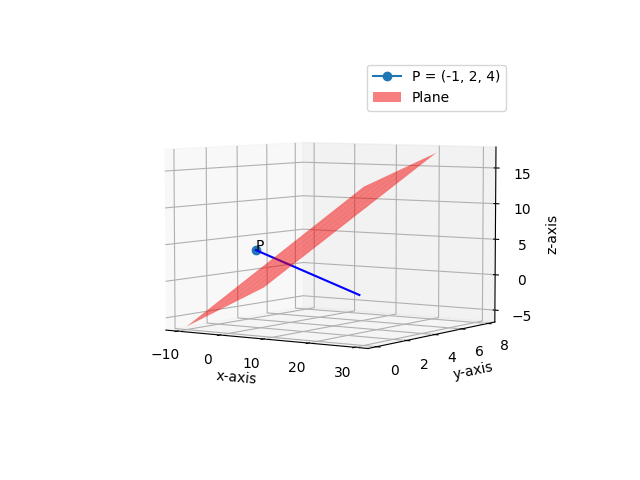
\includegraphics[width = \columnwidth]{Assignment_8.png}
    \caption{Foot of perpendicular from $\myvec{-1 & 2 & 4}$ to the plane $2x +3y -4z +5 = 0$.}
    \label{line and plane}
\end{figure}
\newpage
Verifying solution to \eqref{eq5} with $\textit{least squares}$ method
\begin{align}
	\vec{M}^T(\vec{b} - \vec{M}\vec{x}) &= 0\\
	\label{eq9}\implies \vec{M}^T\vec{M}\vec{x} &= \vec{M}^T\vec{b}
\end{align}
Substituting $\vec{M}, \vec{b}$ from \eqref{eq4} in \eqref{eq9}
\begin{align}
	\myvec{1 & 2 & 0\\0 & 2 & 1}\myvec{1 & 0\\2 & 2\\0 & 1}\vec{x} &= \myvec{1 & 2 & 0\\0 & 2 & 1}\myvec{-2\\1\\\frac{3}{2}}\\
	\myvec{5 & 4\\4 & 5}\myvec{\lambda_1\\\lambda_2} &= \myvec{\frac{-5}{4}\\\frac{17}{8}}\\
	\implies5\lambda_1 + 4\lambda_2&= \frac{-5}{4}\\
	4\lambda_1 + 5\lambda_2&= \frac{17}{8}\\
	\lambda_1 &= \frac{-12499}{10000}\\
	\text{and }\lambda_2 &= \frac{21249}{10000}\\
	\label{eq10}\implies\vec{x} &= \myvec{\frac{-12499}{10000}\\\frac{21249}{10000}}
\end{align}
Comparing \eqref{eq8} and \eqref{eq10} solution is verified.
\end{document}
